\section{Aplikacja webowa}
\label{sec:web-application}

Po konwersji modelu oraz wag na javascriptową wersję biblioteki TensorFlow.js, algorytm bardzo dobrze rozpoznawał statyczne znaki, a dynamiczne ze sporadycznym błędem. W aplikacji estymację pozy dłoni na każdej klatce z kamery robił za nas MediaPipe. Zwracane były również w tym samym stylu co współrzędne punktów nadgarstka, stawów palców oraz dalszych paliczków w pythonowej wersji MediaPipe. Podobnie otrzymano listę współrzędnych relatywnych względem odległości od kamery oraz nadgarstka. W rezultacie, umożliwiło to bezproblemowe odwzorowanie wizualne tych dwóch obiektów, nanosząc ówczesną detekcję na wykrytą rękę oraz podgląd danych do klasyfikacji w postaci przestrzeni trójwymiarowej na wykresie, który umożliwiał na obrót względem osi rzędnej $y$.

Algorytm aplikacji skutecznie odrzucał wyniki poniżej 90\%, aby uniknąć błędnych klasyfikacji, gdy osoba stojąca przed kamerą wykonywała ruch pomiędzy znakami. W momencie wykrycia lewej ręki, kolor punktów wykresu stawał się czerwony i nie dokonywano cyklicznej klasyfikacji, póki przez 30 ostatnich klatek osoba nie pokazała prawej ręki przed kamerą.

\begin{figure}[H]
    \centering
    \begin{subfigure}[H]{0.49\textwidth}
        \centering
        \begin{tikzpicture}
            \begin{axis}[
                    xticklabel style={/pgf/number format/fixed},
                    yticklabel style={/pgf/number format/fixed},
                    zticklabel style={/pgf/number format/fixed},
                ]
                \addplot3[color=connection, mark=*, mark options={fill=landmark}] coordinates {
                        (0.017639633268117905, 0.08171337842941284, 0.03946905583143234)
                        (-0.014130002819001675, 0.06723393499851227, 0.014399375766515732)
                        (-0.03890739381313324, 0.05456604063510895, 0.007250100374221802)
                        (-0.07064789533615112, 0.038058456033468246, 0.002217017114162445)
                        (-0.09892282634973526, 0.024923153221607208,  0.010069653391838074)
                    };
                \addplot3[color=connection, mark=*, mark options={fill=landmark}] coordinates {
                        (-0.030215391889214516, -0.001213383860886097, -0.0006129778921604156)
                        (-0.032151300460100174, -0.032022953033447266, -0.0062715113162994385)
                        (-0.03666038066148758, -0.04995837062597275, -0.01392732560634613)
                        (-0.039656709879636765, -0.06284788250923157, -0.039825428277254105)
                    };
                \addplot3[color=connection, mark=*, mark options={fill=landmark}] coordinates {
                        (-0.0057804579846560955, -0.0046464428305625916, 0.003999499604105949)
                        (0.001754043623805046, -0.015449277125298977, -0.031981803476810455)
                        (-0.00266991276293993, 0.009595227427780628, -0.042030736804008484)
                        (-0.010893994942307472, 0.019357839599251747, -0.020213454961776733)
                    };
                \addplot3[color=connection, mark=*, mark options={fill=landmark}] coordinates {
                        (0.018689550459384918, -0.0016619960078969598, 0.0020418018102645874)
                        (0.020380061119794846, -0.002630592091009021, -0.03321712464094162)
                        (0.013807661831378937, 0.023050721734762192, -0.03517334163188934)
                        (0.005579805001616478, 0.033607468008995056, -0.013853594660758972)
                    };
                \addplot3[color=connection, mark=*, mark options={fill=landmark}] coordinates {
                        (0.037820134311914444, 0.015773072838783264, 0.00044389069080352783)
                        (0.043130062520504, 0.005058330949395895, -0.021947376430034637)
                        (0.03323442488908768, 0.01886684261262417, -0.03341059386730194)
                        (0.020432576537132263, 0.03217173367738724, -0.01788344979286194)
                    };
                \addplot3[color=connection, mark=*, mark options={fill=landmark}] coordinates {
                        (0.017639633268117905, 0.08171337842941284, 0.03946905583143234)
                        (-0.030215391889214516, -0.001213383860886097, -0.0006129778921604156)
                        (-0.0057804579846560955, -0.0046464428305625916, 0.003999499604105949)
                        (0.018689550459384918, -0.0016619960078969598, 0.0020418018102645874)
                        (0.037820134311914444, 0.015773072838783264, 0.00044389069080352783)
                        (0.017639633268117905, 0.08171337842941284, 0.03946905583143234)
                    };
            \end{axis}
        \end{tikzpicture}
        \caption{Znak \enquote{L}}
        \label{fig:l-landmarks}
    \end{subfigure}
    \begin{subfigure}[H]{0.49\textwidth}
        \centering
        \begin{tikzpicture}
            \begin{axis}[
                    xticklabel style={/pgf/number format/fixed},
                    yticklabel style={/pgf/number format/fixed},
                    zticklabel style={/pgf/number format/fixed},
                ]
                \addplot3[color=connection, mark=*, mark options={fill=landmark}] coordinates {
                        (0.02536553516983986, 0.08305147290229797, 0.02005057781934738)
                        (0.00019600242376327515, 0.06300190836191177, 0.03042314574122429)
                        (-0.024719681590795517, 0.04531867802143097, 0.03204931318759918)
                        (-0.050325680524110794, 0.02942325733602047, 0.028932515531778336)
                        (-0.06961864233016968, 0.013104964978992939, 0.021967247128486633)
                    };
                \addplot3[color=connection, mark=*, mark options={fill=landmark}] coordinates {
                        (-0.013172917999327183, -0.002788574667647481, 0.02529831975698471)
                        (-0.03621090203523636, -0.008697057142853737, 0.012233812361955643)
                        (-0.055835019797086716, -0.006854263134300709, 0.008941886015236378)
                        (-0.07483062893152237, 0.002718396484851837, -0.0027886182069778442)
                    };
                \addplot3[color=connection, mark=*, mark options={fill=landmark}] coordinates {
                        (-0.0012524011544883251, -0.0038268975913524628, 0.005632670596241951)
                        (-0.03063426911830902, -0.011562779545783997, -0.006345808506011963)
                        (-0.053872670978307724, 0.001530245877802372, -0.010041758418083191)
                        (-0.07048270106315613, 0.010363458655774593, -0.0074196308851242065)
                    };
                \addplot3[color=connection, mark=*, mark options={fill=landmark}] coordinates {
                        (0.007995815016329288, -0.00042493839282542467, -0.01622706651687622)
                        (-0.01960957609117031, -0.0005572536028921604, -0.022953476756811142)
                        (-0.04288184642791748, 0.00571034848690033, -0.02329181134700775)
                        (-0.060070380568504333, 0.011484622955322266, -0.023675478994846344)
                    };
                \addplot3[color=connection, mark=*, mark options={fill=landmark}] coordinates {
                        (0.011657901108264923, 0.01594752073287964, -0.030137792229652405)
                        (-0.007262116298079491, 0.013314315117895603, -0.03623213618993759)
                        (-0.028852315619587898, 0.01018589735031128, -0.03668694198131561)
                        (-0.046098820865154266, 0.013425415381789207, -0.04154990613460541)
                    };
                \addplot3[color=connection, mark=*, mark options={fill=landmark}] coordinates {
                        (0.02536553516983986, 0.08305147290229797, 0.02005057781934738)
                        (-0.013172917999327183, -0.002788574667647481, 0.02529831975698471)
                        (-0.0012524011544883251, -0.0038268975913524628, 0.005632670596241951)
                        (0.007995815016329288, -0.00042493839282542467, -0.01622706651687622)
                        (0.011657901108264923, 0.01594752073287964, -0.030137792229652405)
                        (0.02536553516983986, 0.08305147290229797, 0.02005057781934738)
                    };
            \end{axis}
        \end{tikzpicture}
        \caption{Znak \enquote{E}}
        \label{fig:e-landmarks}
    \end{subfigure}
    \caption{Koordynaty stawów prawej ręki}
    \label{fig:hand-landmarks}
\end{figure}

\begin{figure}[H]
    \centering
    \begin{subfigure}{\textwidth}
        \centering
        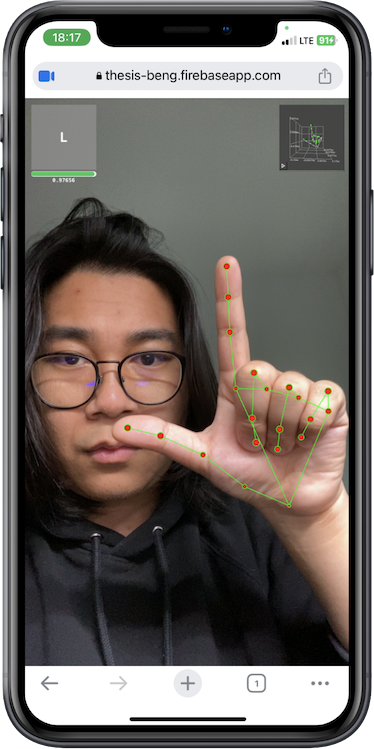
\includegraphics[width=0.3\textwidth]{figures/mobile}
        \caption{Wersja mobilna}
        \label{fig:mobile-mockup}
        \vspace{1cm}
    \end{subfigure}
    \begin{subfigure}{\textwidth}
        \centering
        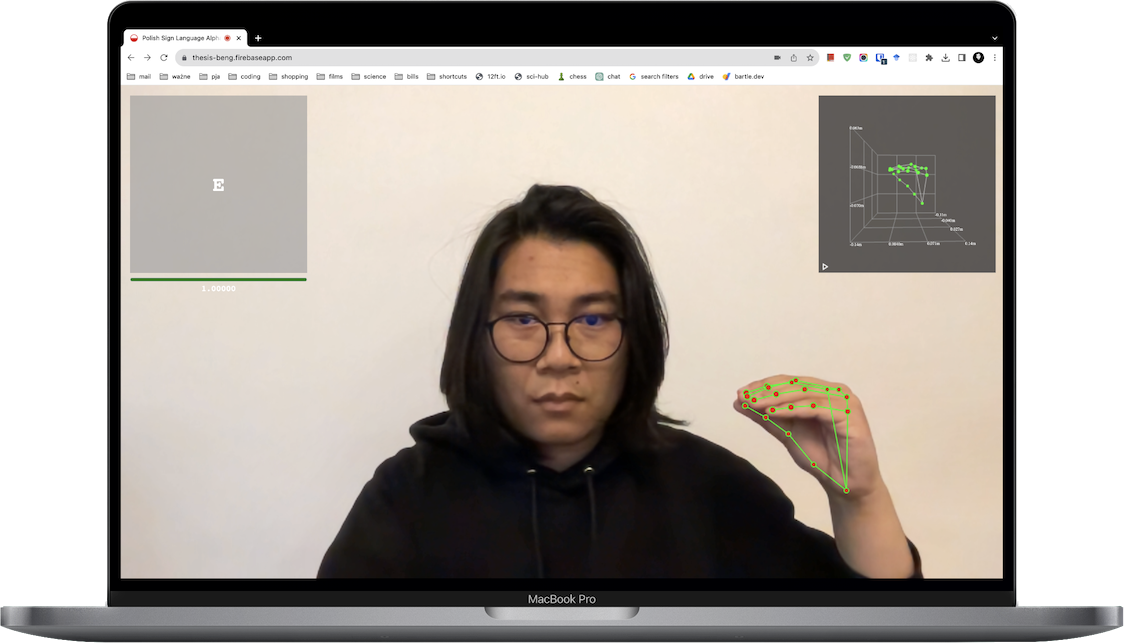
\includegraphics[width=\textwidth]{figures/desktop}
        \caption{Wersja desktopowa}
        \label{fig:desktop-mockup}
    \end{subfigure}
    \caption{Makiety aplikacji}
    \label{fig:mockups}
\end{figure}

Model początkowo dokonywał klasyfikacji co 50 milisekund. Obserwacje wersji testowej wykazały wolniejsze działanie aplikacji, a konsekwencją zbyt częstego wykonania były przypadkowe klasyfikacje znaków dynamicznych między zmianami układu palców.

\begin{listing}[H]
    \color{white}
    \begin{minted}[label=predictor.js]{javascript}
export class Predictor {
    constructor() {
        this.sequences = [];
        this.sign = "";
        this.accuracy = 0;
    }

    async init() {
        try {
            this.model = await loadLayersModel("model.json");
            this.predict = this.throttle(500);
        } catch (error) {
            console.error(error);
        }
    }

    shiftSequences(multiHandedness, multiHandWorldLandmarks) {
        const enoughFrames = this.sequences.length === 30;

        if (enoughFrames) this.sequences.shift();

        const rightHandIndex = this.getRightHandIndex(multiHandedness);
        const landmarks = rightHandIndex !== -1 ? multiHandWorldLandmarks[rightHandIndex] : [];
        const sequence = landmarks.map((landmark) => [landmark.x, landmark.y, landmark.z]).flat();

        this.sequences.push(sequence);
        const noneEmpty = this.sequences.every((sequence) => sequence.length === 63);

        if (!enoughFrames || !noneEmpty) return;

        this.predict(0.9);
    }

    throttle(delay) {
        this.predictionTime = Date.now();

        return (threshold) => {
            let now = Date.now();

            if (now - this.predictionTime > delay) {
                this.predictionTime = now;
                const tensor = this.model.predict(tensor3d([this.sequences]));
                const [predictions] = tensor.arraySync();
                const topAccuracy = Math.max(...predictions);
                const prediction = alphabet[predictions.indexOf(topAccuracy)];

                if (topAccuracy >= threshold) {
                    this.sign = prediction;
                    this.accuracy = topAccuracy;
                }
            }
        };
    }

    getRightHandIndex(multiHandedness) {
        return multiHandedness.findIndex((handedness) => handedness.label === "Right");
    }
}
    \end{minted}
    \caption{Algorytm klasyfikacji}
    \label{lst:classification-algorithm}
\end{listing}

Ostatecznie w aplikacji dokonywano klasyfikacji sekwencji współrzędnych co 500 milisekund, przez co nie obciążono zasobów obliczeniowych. Dzięki tej drobnej zmianie, czas na reakcję był odpowiedni, aby w międzyczasie zmienić ustawienie palców.
